\documentclass[11pt,a4paper,twoside]{article}

\usepackage[utf8]{inputenc}
\usepackage[T1]{fontenc}
\usepackage{lmodern}
\usepackage{geometry}
\geometry{margin=1.1in}
\usepackage{graphicx}
\usepackage{float}
\usepackage{hyperref}
\usepackage{xcolor}
\usepackage{listings}
\usepackage{fancyhdr}
\usepackage{booktabs}
\usepackage{caption}
\usepackage{parskip}
\usepackage{abstract}
\usepackage{titlesec}

% ── Colors ───────────────────────────────────────────────────────────
\definecolor{sysblue}{HTML}{1E3A8A}
\definecolor{sysgray}{HTML}{4B5563}
\definecolor{codebg}{HTML}{F9FAFB}

% ── Code listing style ───────────────────────────────────────────────
\lstdefinestyle{academic}{
    backgroundcolor=\color{codebg},
    basicstyle=\ttfamily\footnotesize,
    breaklines=true,
    frame=tb,
    rulecolor=\color{sysgray!40},
    xleftmargin=8pt,
    xrightmargin=8pt,
    aboveskip=12pt,
    belowskip=12pt,
    showstringspaces=false,
}
\lstset{style=academic}

% ── Headers / formatting ────────────────────────────────────────────
\hypersetup{
    colorlinks=true,
    linkcolor=sysblue,
    urlcolor=sysblue,
    citecolor=sysblue,
}

\pagestyle{fancy}
\fancyhf{}
\fancyhead[LE,RO]{\thepage}
\fancyhead[LO]{\textsl{PipeRewind: A Time-Travel Debugger for UNIX Pipelines}}
\fancyhead[RE]{\textsl{L. Takahashi, E. Chavez}}
\renewcommand{\headrulewidth}{0.4pt}

\titleformat{\section}{\large\bfseries\color{sysblue}}{\thesection}{1em}{}
\titleformat{\subsection}{\normalsize\bfseries}{\thesubsection}{1em}{}

% ── Title ────────────────────────────────────────────────────────────
\title{
    \vspace{-1.5cm}
    \textbf{\Large PipeRewind: A Time-Travel Debugger for UNIX Shell Pipelines}\\
    \large Systems Programming Architecture Report
}
\author{
    Luiz Takahashi \quad \& \quad Ehzoc Chavez\\
    \small\textit{Washington State University}
}
\date{\vspace{-3ex}}

\begin{document}
\maketitle
\thispagestyle{empty}

% ━━━━━━━━━━━━━━━━━━━━━━━━━━━━━━━━━━━━━━━━━━━━━━━━━━━━━━━━━━━━━━━━━━
\begin{abstract}
\noindent
UNIX shell pipelines rely on anonymous inter-process communication (IPC) channels, traditionally rendering intra-pipeline data transmission unobservable without pervasive source code modification or system call tracing. This paper introduces PipeRewind, a deterministic execution logger and time-travel debugger that seamlessly interposes on process pipelines. By utilizing \texttt{dup2} file descriptor redirection in conjunction with an \texttt{epoll}-driven asynchronous capture loop, PipeRewind multiplexes and serializes standard I/O streams into an indexed binary trace sequence. The system introduces an \texttt{ncurses}-based interactive visualization environment equipped with a sliding-window data cache and real-time process state polling via the \texttt{/proc} pseudo-filesystem, enabling high-fidelity replay of process executions without exhausting memory bounds. 
\end{abstract}
% ━━━━━━━━━━━━━━━━━━━━━━━━━━━━━━━━━━━━━━━━━━━━━━━━━━━━━━━━━━━━━━━━━━

\section{Introduction}

The modularity of the UNIX pipeline (\texttt{|}) abstraction allows developers to compose complex text-processing operations from minimal, specialized utilities. However, the standard behavior of linking standard output (\texttt{STDOUT\_FILENO}) of process $P_i$ to standard input (\texttt{STDIN\_FILENO}) of process $P_{i+1}$ via contiguous kernel pipe buffers results in extreme operational opacity. If a data corruption or failure anomaly occurs within an intermediate pipeline stage, debugging necessitates ad-hoc injection of \texttt{tee} commands or reliance on high-overhead diagnostic utilities such as \texttt{strace}, which injects significant noise via kernel context boundary intersections.

\textbf{PipeRewind} addresses this deficiency by establishing a transparent virtualization layer atop the standard pipeline semantic model. Rather than direct process-to-process bridging, PipeRewind acts as a multiplexed data broker. It intercepts arbitrary textual byte streams across $N$ executing processes, serializes exact temporal events via POSIX high-resolution clocks, and persists the payload into an actionable \texttt{.prt} binary artifact for deferred or real-time inspection.

\section{System Architecture and Process Topology}

The instantiation of the PipeRewind trace involves establishing a rigorous inter-process topology orchestrated by a primary Capture Engine parent process.

\subsection{Process Hierarchy \& FD Redirection}

Figure~\ref{fig:hierarchy} illustrates the \texttt{fork()} and \texttt{exec()} lifecycle deployed for dynamic command execution. For an $N$-stage pipeline, the Capture Engine provisions $2(N-1) + 1$ anonymous pipe file descriptors. 

Prior to executing the binary payload via \texttt{execvp()}, the child process environment undergoes descriptor redirection. For pipeline stage $P_i$, the child invokes \texttt{dup2()} to aggressively overwrite \texttt{STDIN\_FILENO} with the read-end of the inbound capture pipe, and \texttt{STDOUT\_FILENO} with the write-end of the outbound capture pipe. The child's residual file descriptors are rigorously closed to prevent internal descriptor leaking or inadvertent blocking architectures.

\begin{figure}[H]
    \centering
    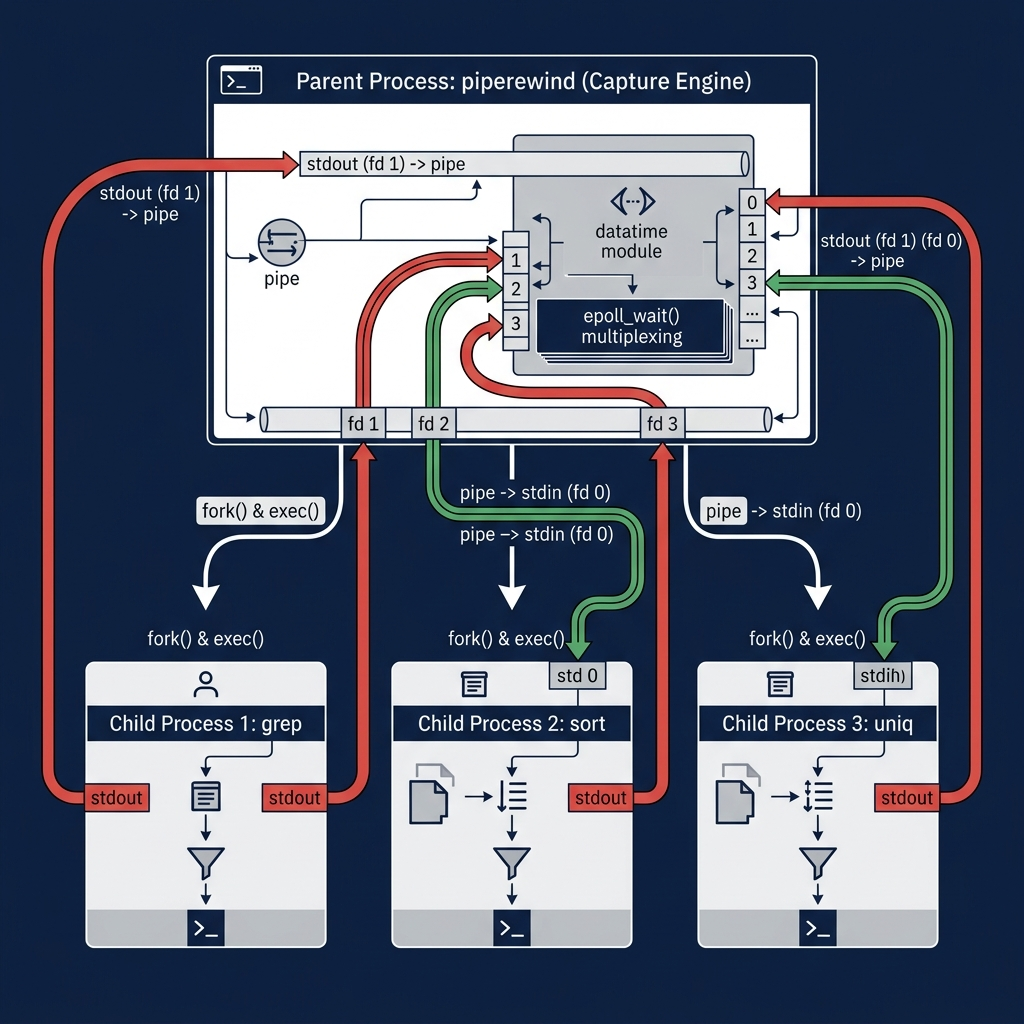
\includegraphics[width=0.85\textwidth]{images/technical/process_hierarchy.png}
    \caption{Process hierarchy and file descriptor abstraction. The Capture Engine interfaces via bridged pipes rather than allowing direct kernel IPC between children.}
    \label{fig:hierarchy}
\end{figure}

\subsection{Asynchronous I/O via \texttt{epoll}}

Linearly polling or blocking on individual pipe \texttt{read()} operations would inherently deadlock complex execution trees due to kernel pipe capacity limitations ($64\,\mathrm{KB}$ typically) and divergent process scheduling behavior.

Consequently, PipeRewind leverages the horizontal trigger mechanisms of \texttt{epoll}. The Capture Engine registers the read-ends of all $P_i$ output pipes into the epoll instance. Adhering strictly to non-blocking I/O paradigms (\texttt{O\_NONBLOCK}), the system enters an \texttt{epoll\_wait()} multiplexing loop. When data is flushed by any process $P_i$, the engine is awakened, drains the descriptor buffer into user-space, tags it with a monotonic nanosecond timestamp, and propagates the payload to the $P_{i+1}$ input pipe.

\begin{figure}[H]
    \centering
    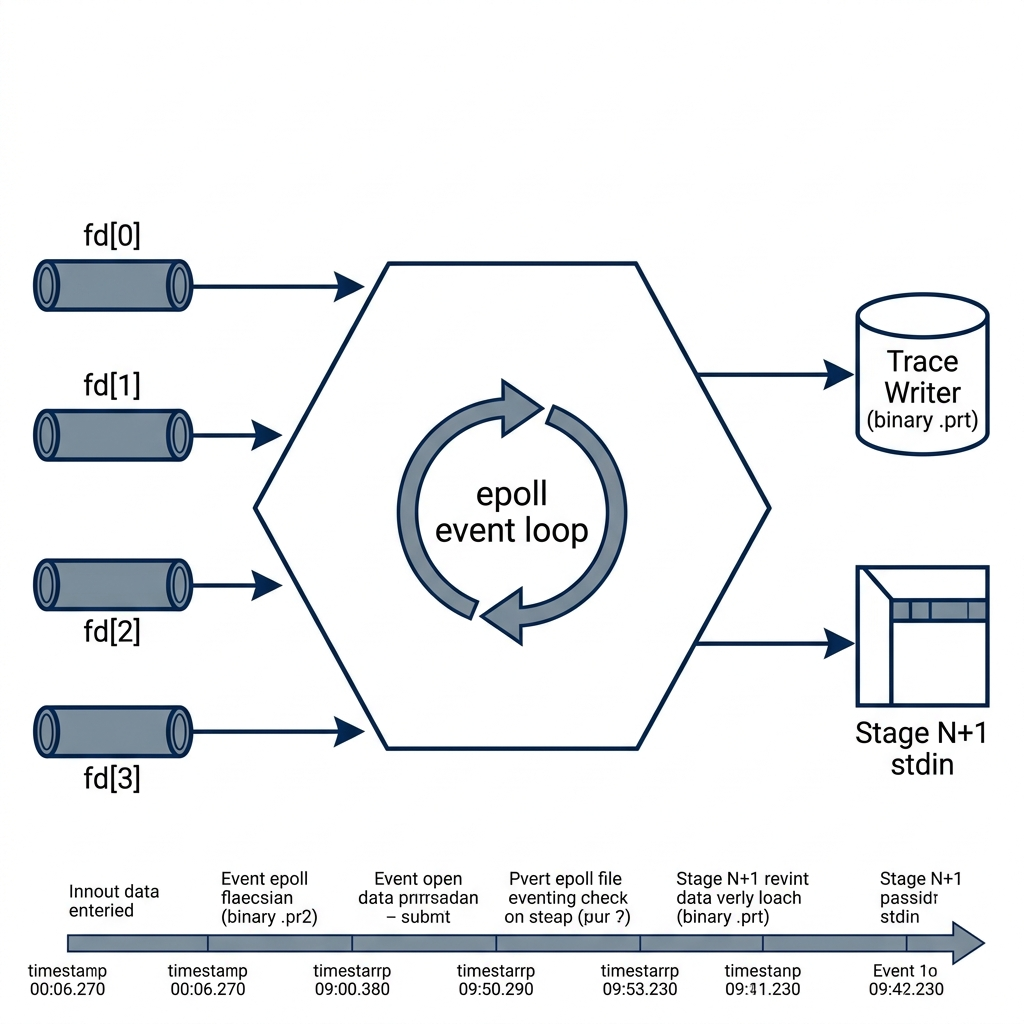
\includegraphics[width=0.8\textwidth]{images/technical/epoll_architecture.png}
    \caption{Event-driven architecture: The \texttt{epoll} event loop concurrently manages inbound buffers ($fd_n$), forwarding data structurally while serializing execution state into the Binary Trace Writer.}
    \label{fig:epoll}
\end{figure}

\section{Data Persistence and Deterministic Representation}

To facilitate accurate `time-travel' replay capabilities without re-executing transient side-effecting binary trees, the sequence is serialized into the \texttt{.prt} binary schema.

A \texttt{.prt} trace minimizes serialization overhead by operating fundamentally upon binary structs written contiguously via \texttt{fwrite()}. The layout consists of:
\begin{enumerate}
    \item \textbf{File Header}: Global topology definitions and endian-verification magic numbers.
    \item \textbf{Stage Directories}: Process Command-Line Arguments, PID metrics, and associated metadata strings.
    \item \textbf{Event Stream}: Interleaved, chronologically-ordered polymorphic blocks representing kernel-state changes.
    \item \textbf{Payload Indexing Lookup}: A terminal indexing table providing \texttt{fseek()} localized byte-offsets mapping directly to individual sequence indices $T_i$, bypassing $O(N)$ sequential parses on massive filesides.
\end{enumerate}

Recorded states include \texttt{PROC\_START}, \texttt{PROC\_EXIT}, \texttt{PIPE\_EOF}, \texttt{DATA\_IN}, and \texttt{DATA\_OUT}.

\section{Interactive Replay and Sliding-Window Caching}

The core feature of PipeRewind is the \texttt{ncurses}-powered \texttt{tui.c} terminal viewer. Traditional text-visualizers succumb to out-of-memory (OOM) faults when ingesting extensive pipeline captures. 

PipeRewind circumvents heap explosion through the implementation of a constrained \textbf{sliding-window caching} heuristic. While the \texttt{.prt} artifact is mapped structurally, payloads are actively \texttt{calloc}ed mapping solely bounded subsets consisting of a localized parameter array (defaulting strictly to $20,000$ adjacent sequential transactions). 

\begin{figure}[H]
    \centering
    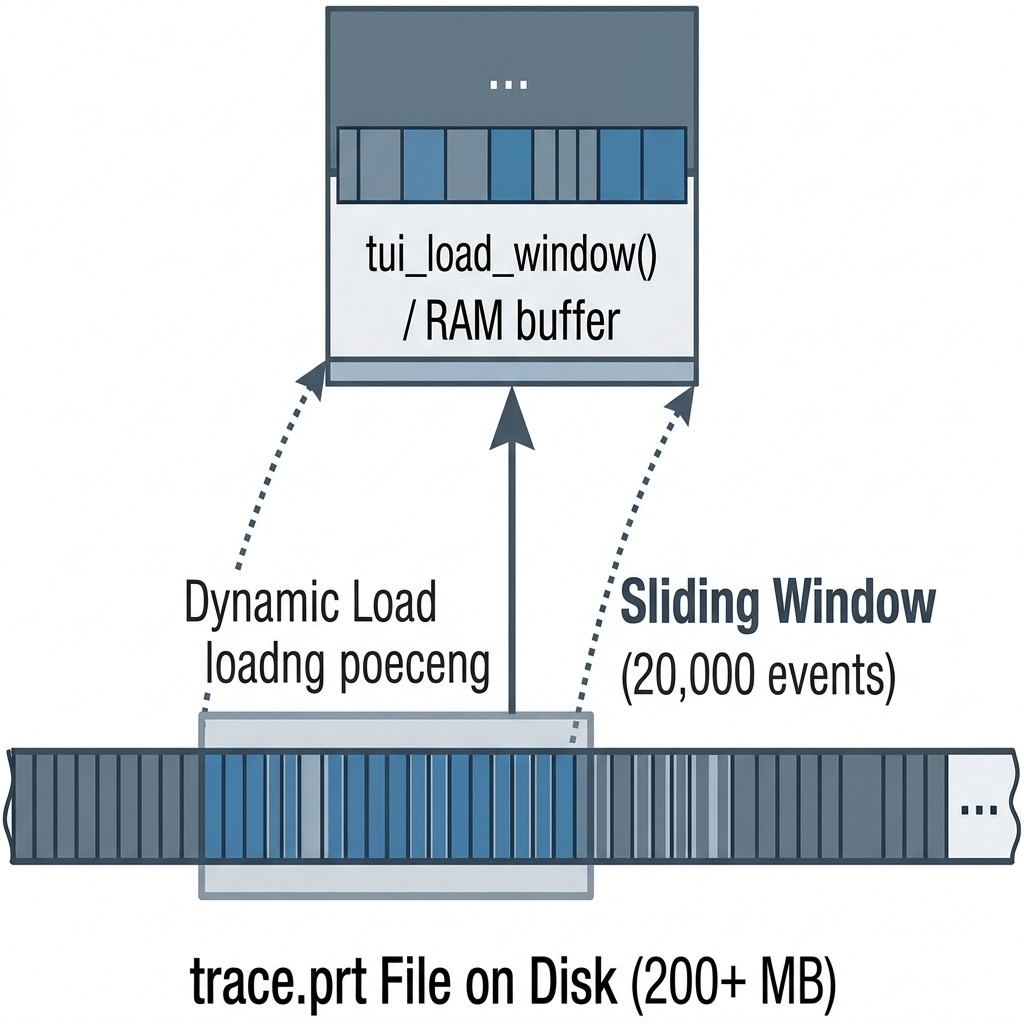
\includegraphics[width=0.75\textwidth]{images/technical/sliding_window.png}
    \caption{Sliding window trace access model: Raw \texttt{.prt} disk payloads are dynamically hoisted into memory sequentially as required by TUI navigational directives.}
    \label{fig:window}
\end{figure}

As navigational index pointers surpass the localized RAM boundary restrictions, dynamic destruction sequence vectors automatically \texttt{free()} stale heuristic events and recursively perform localized chunk loading.

\section{Live Attachment Methodology}
Advancing beyond postmortem trace evaluation, PipeRewind integrates a \texttt{live} daemon protocol. The core Capture Engine \texttt{epoll} abstraction is wrapped inside an orthogonal detached \texttt{pthread}, rendering raw events directly to the \texttt{trace.prt} handler buffer securely. Simultaneously, the TUI loop spins up on the prime directive mapping dynamic file expansion events efficiently through \texttt{trace\_reader\_refresh()} array reallocation logic, bridging temporal pipeline monitoring securely inside execution context frameworks with asynchronous synchronization parameters.

\section{Conclusion}

PipeRewind establishes a formidable enhancement over standard UNIX pipeline debugging architectures. By strictly adhering to event-driven C99 design paradigms, mastering file descriptor redirection via POSIX specifications, and employing dynamic index-constrained UI paradigms, it grants engineers granular visibility into asynchronous multiprocess text streams without incurring untenable memory faults or altering underlying kernel structures.

\vfill
\begin{center}
\small \textbf{Repository URL:} \url{https://github.com/balloonjazz/Pipe-Rewind}
\end{center}

\end{document}
